\chapter{Desarrollo}
\label{hardware}

\section{Búsqueda de información}
\label{busqueda_informacion}

El primer paso es identificar el hardware del que disponemo en la fábrica con ayuda de las fotos tomadas:
    \begin{figure}[H]
            \centering
            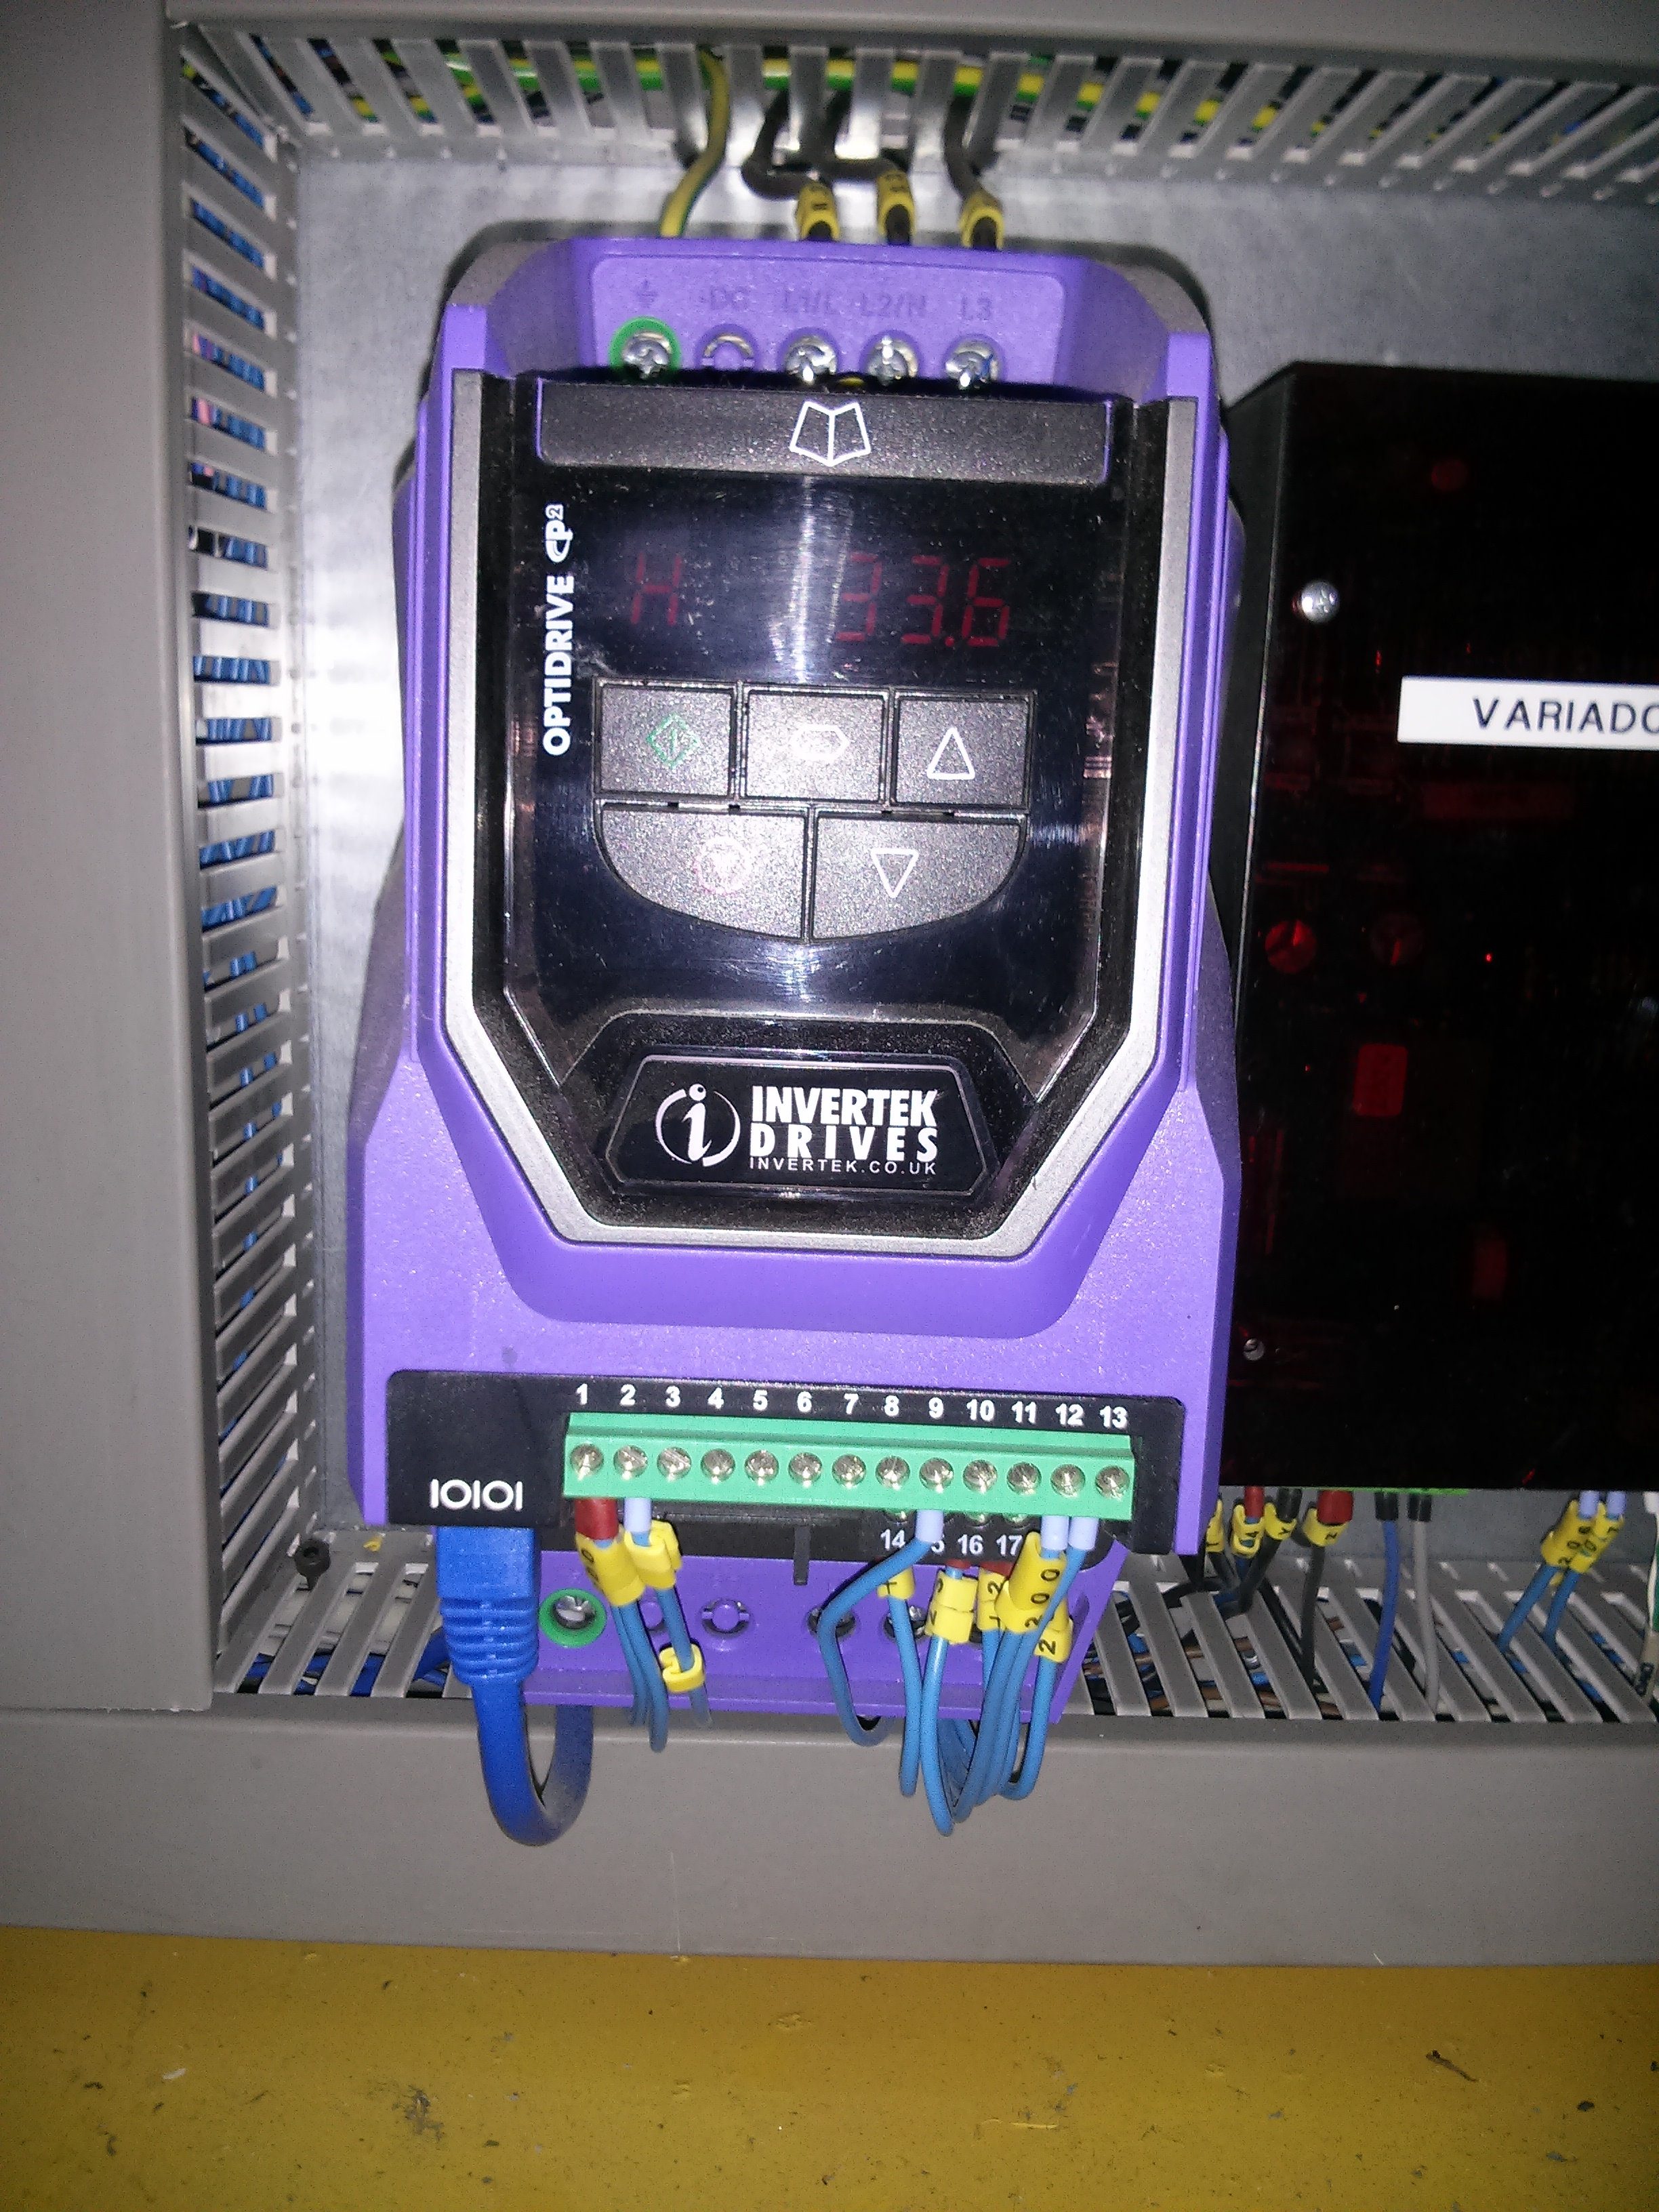
\includegraphics[width=0.4\textwidth]{images/huesca/IMG_20141216_174810.jpg}
            \caption{Variador Optidrive}
            \label{fig:hardware_variador}
    \end{figure}

    \begin{figure}[H]
            \centering
            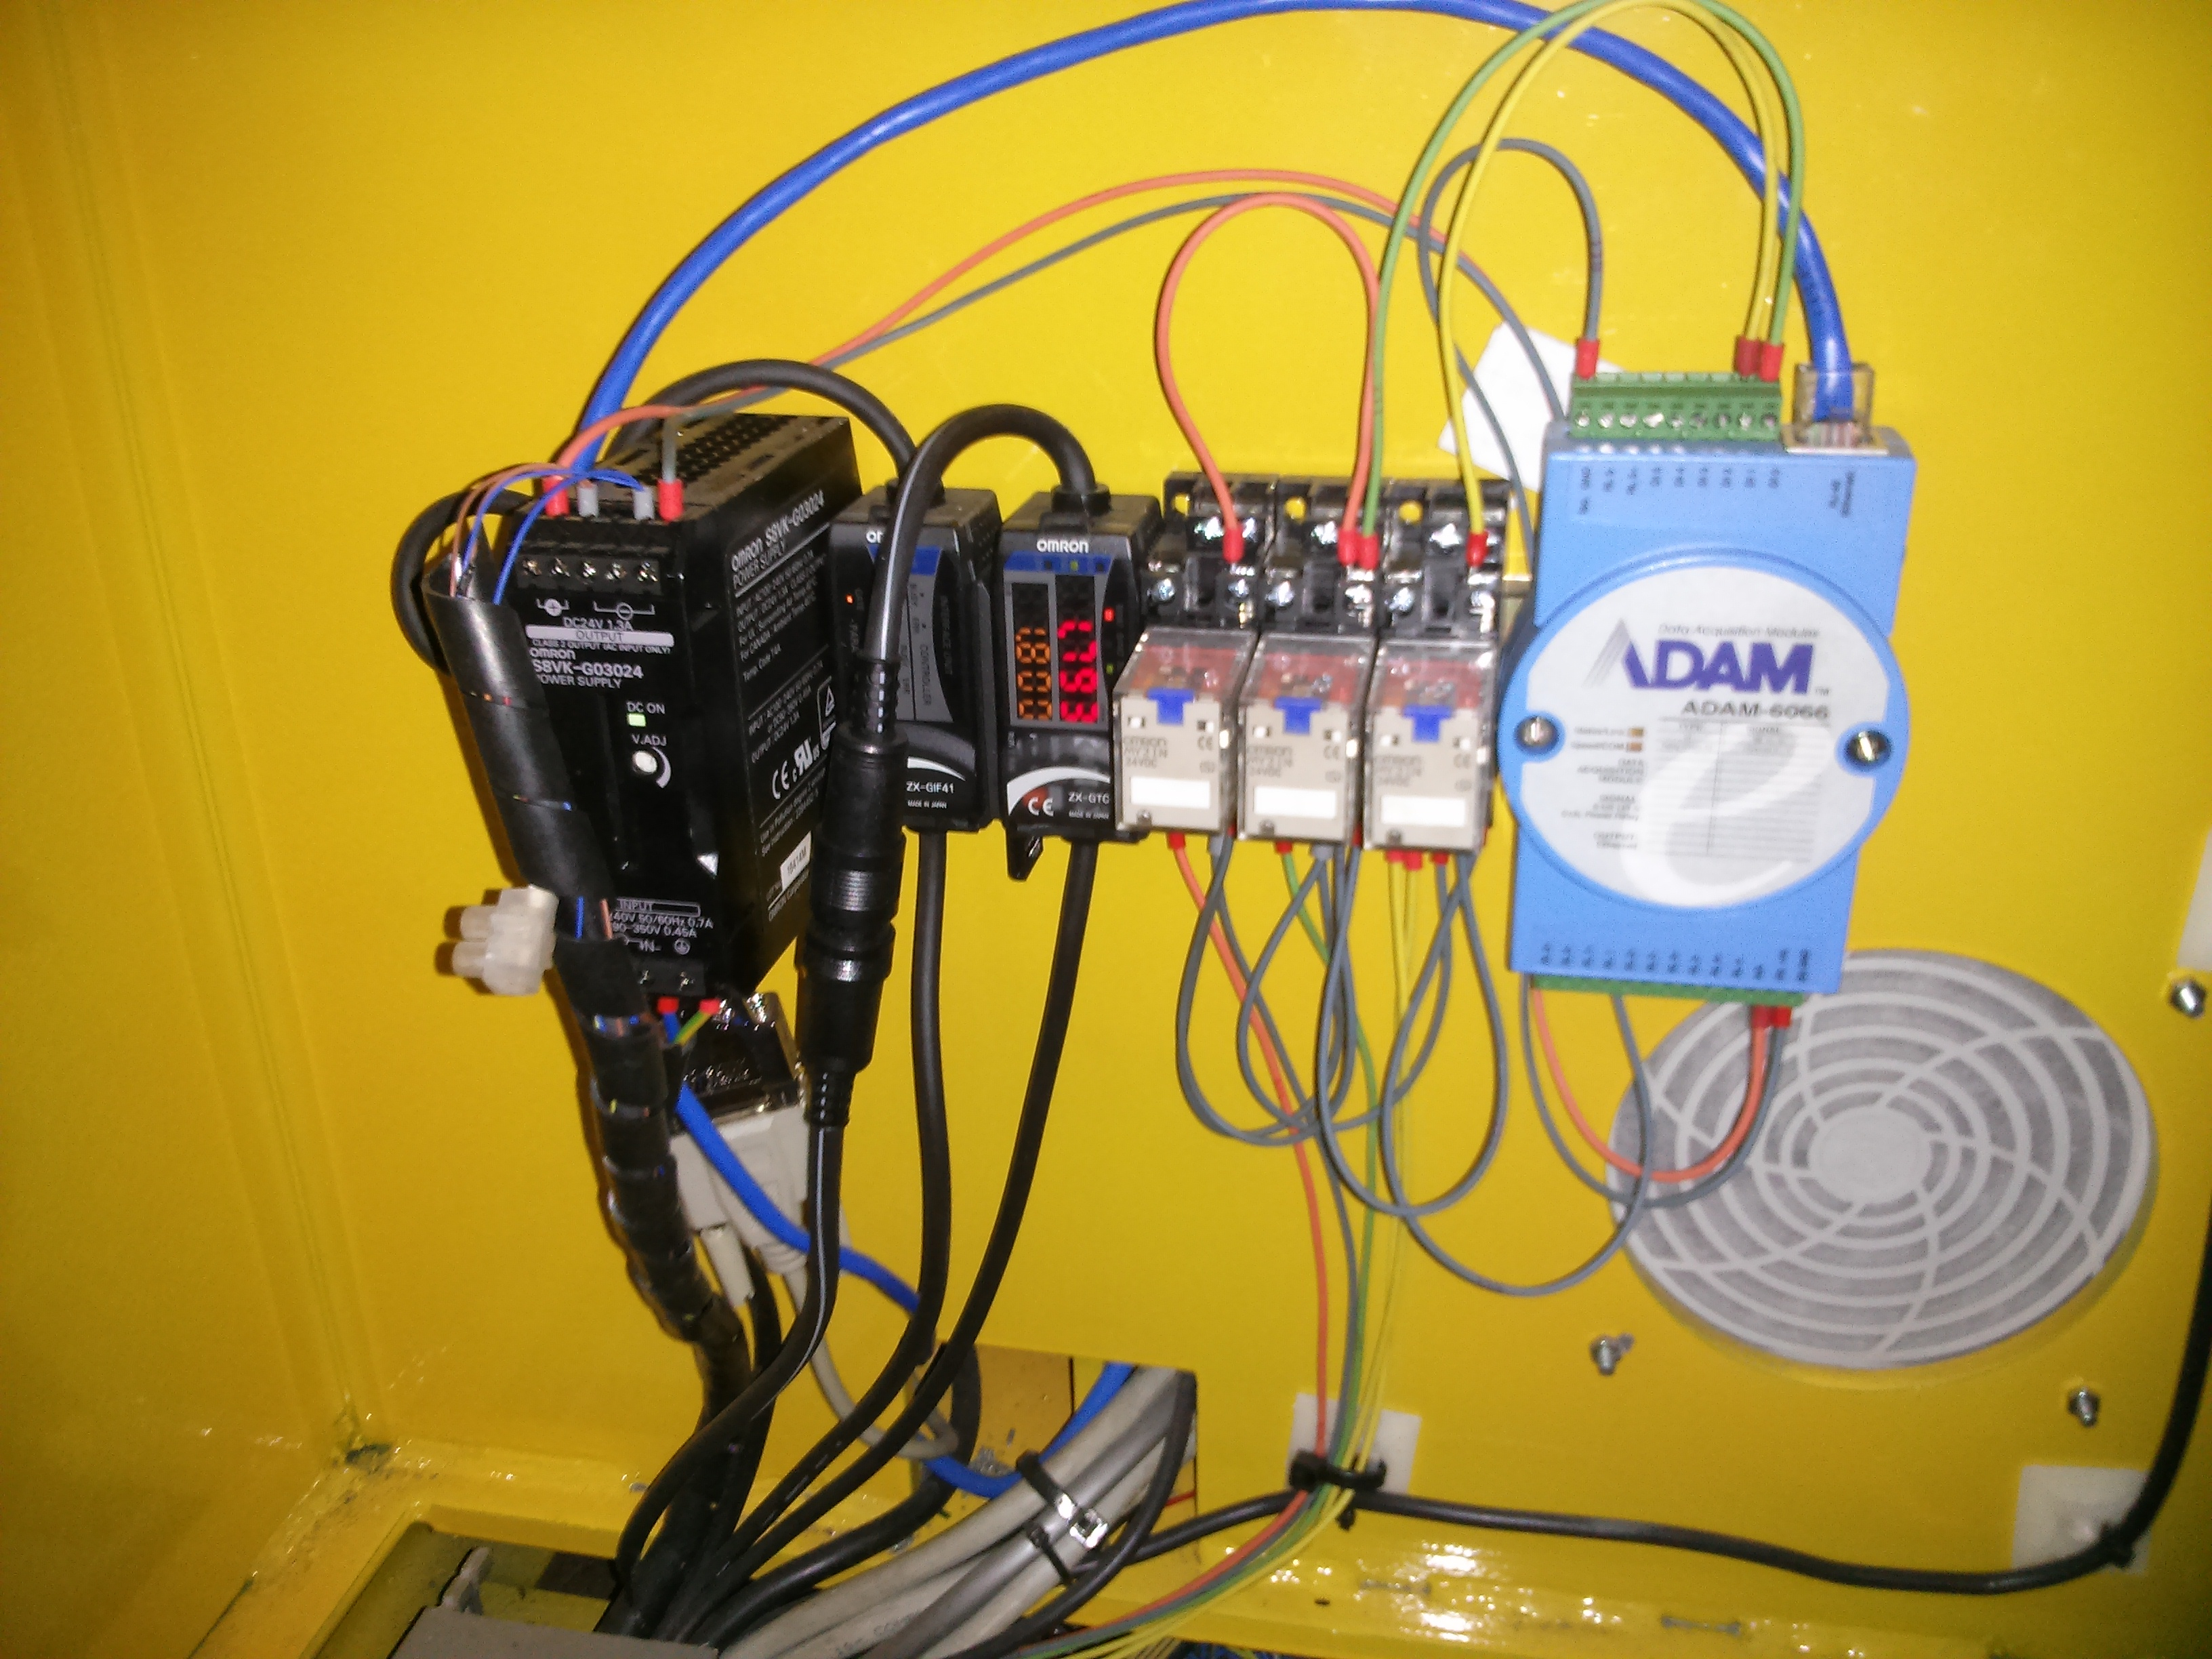
\includegraphics[width=0.4\textwidth]{images/huesca/IMG_20141216_174824.jpg}
            \caption{Sensor de diámetro y perifería}
            \label{fig:hardware_diametro}
    \end{figure}

    \begin{figure}[H]
            \centering
            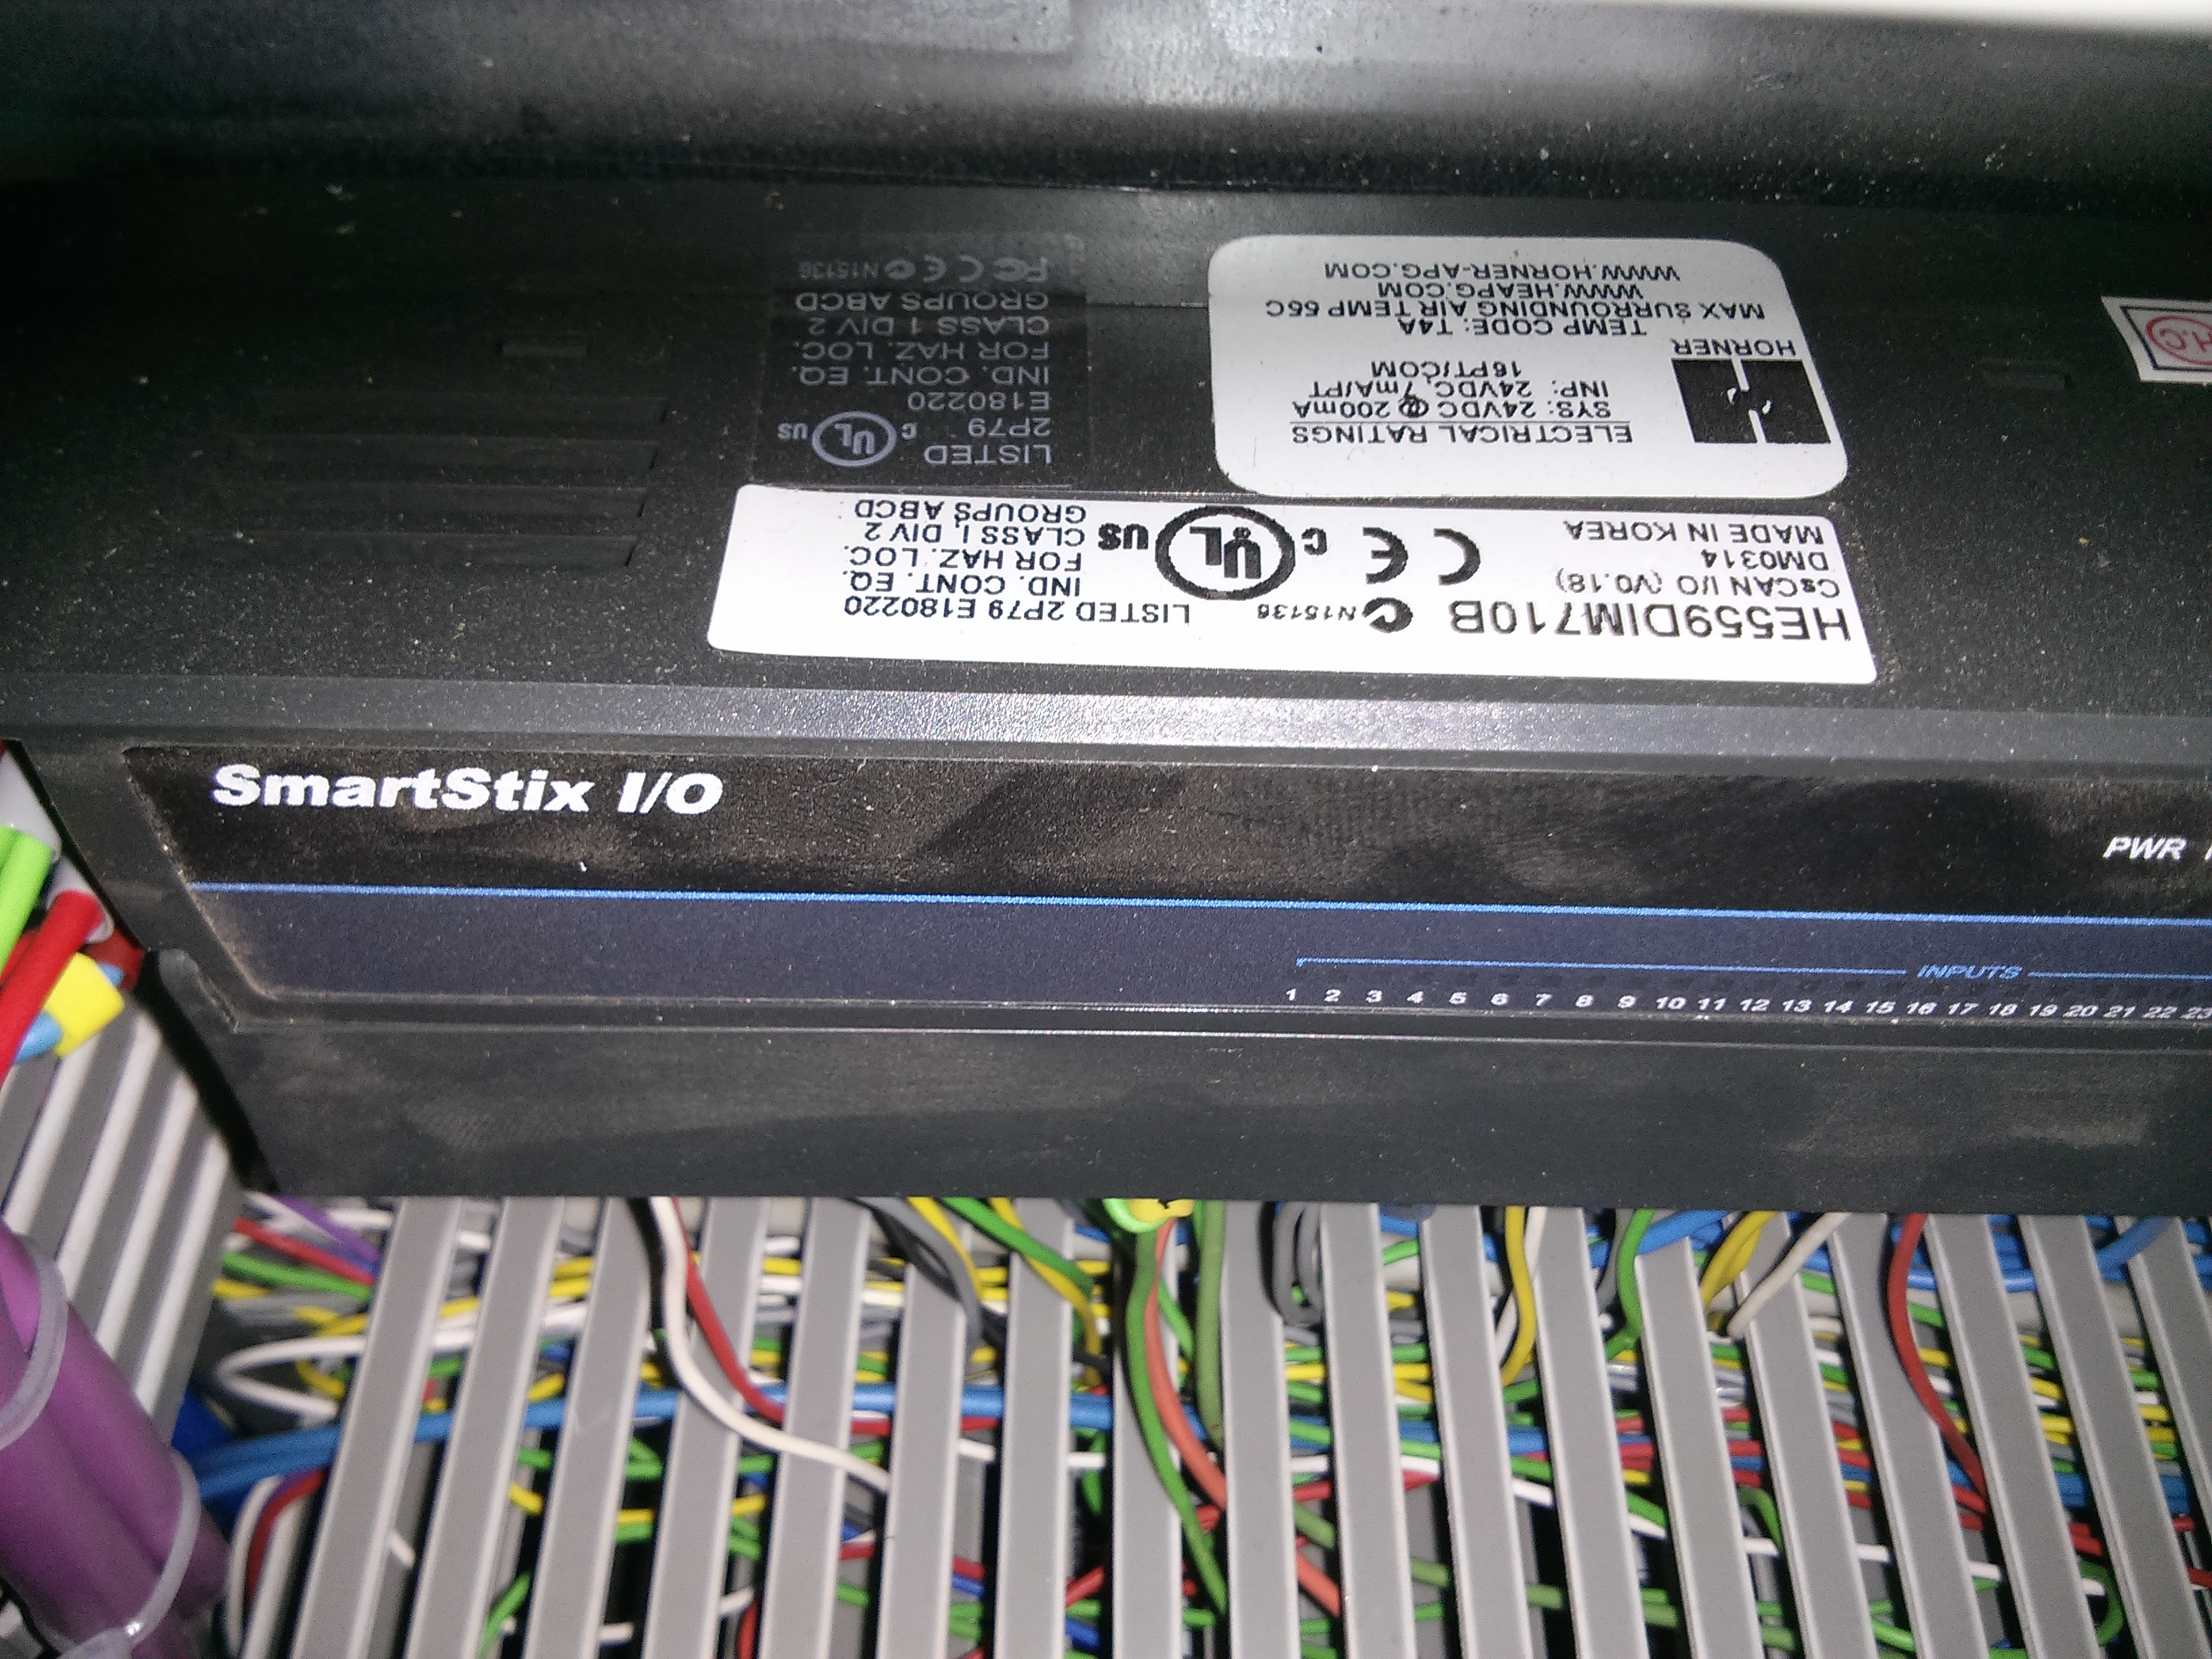
\includegraphics[width=0.4\textwidth]{images/huesca/IMG_20141216_174925.jpg}
            \caption{Perifería distribuida}
            \label{fig:hardware_periferia}
    \end{figure}

    \begin{figure}[H]
            \centering
            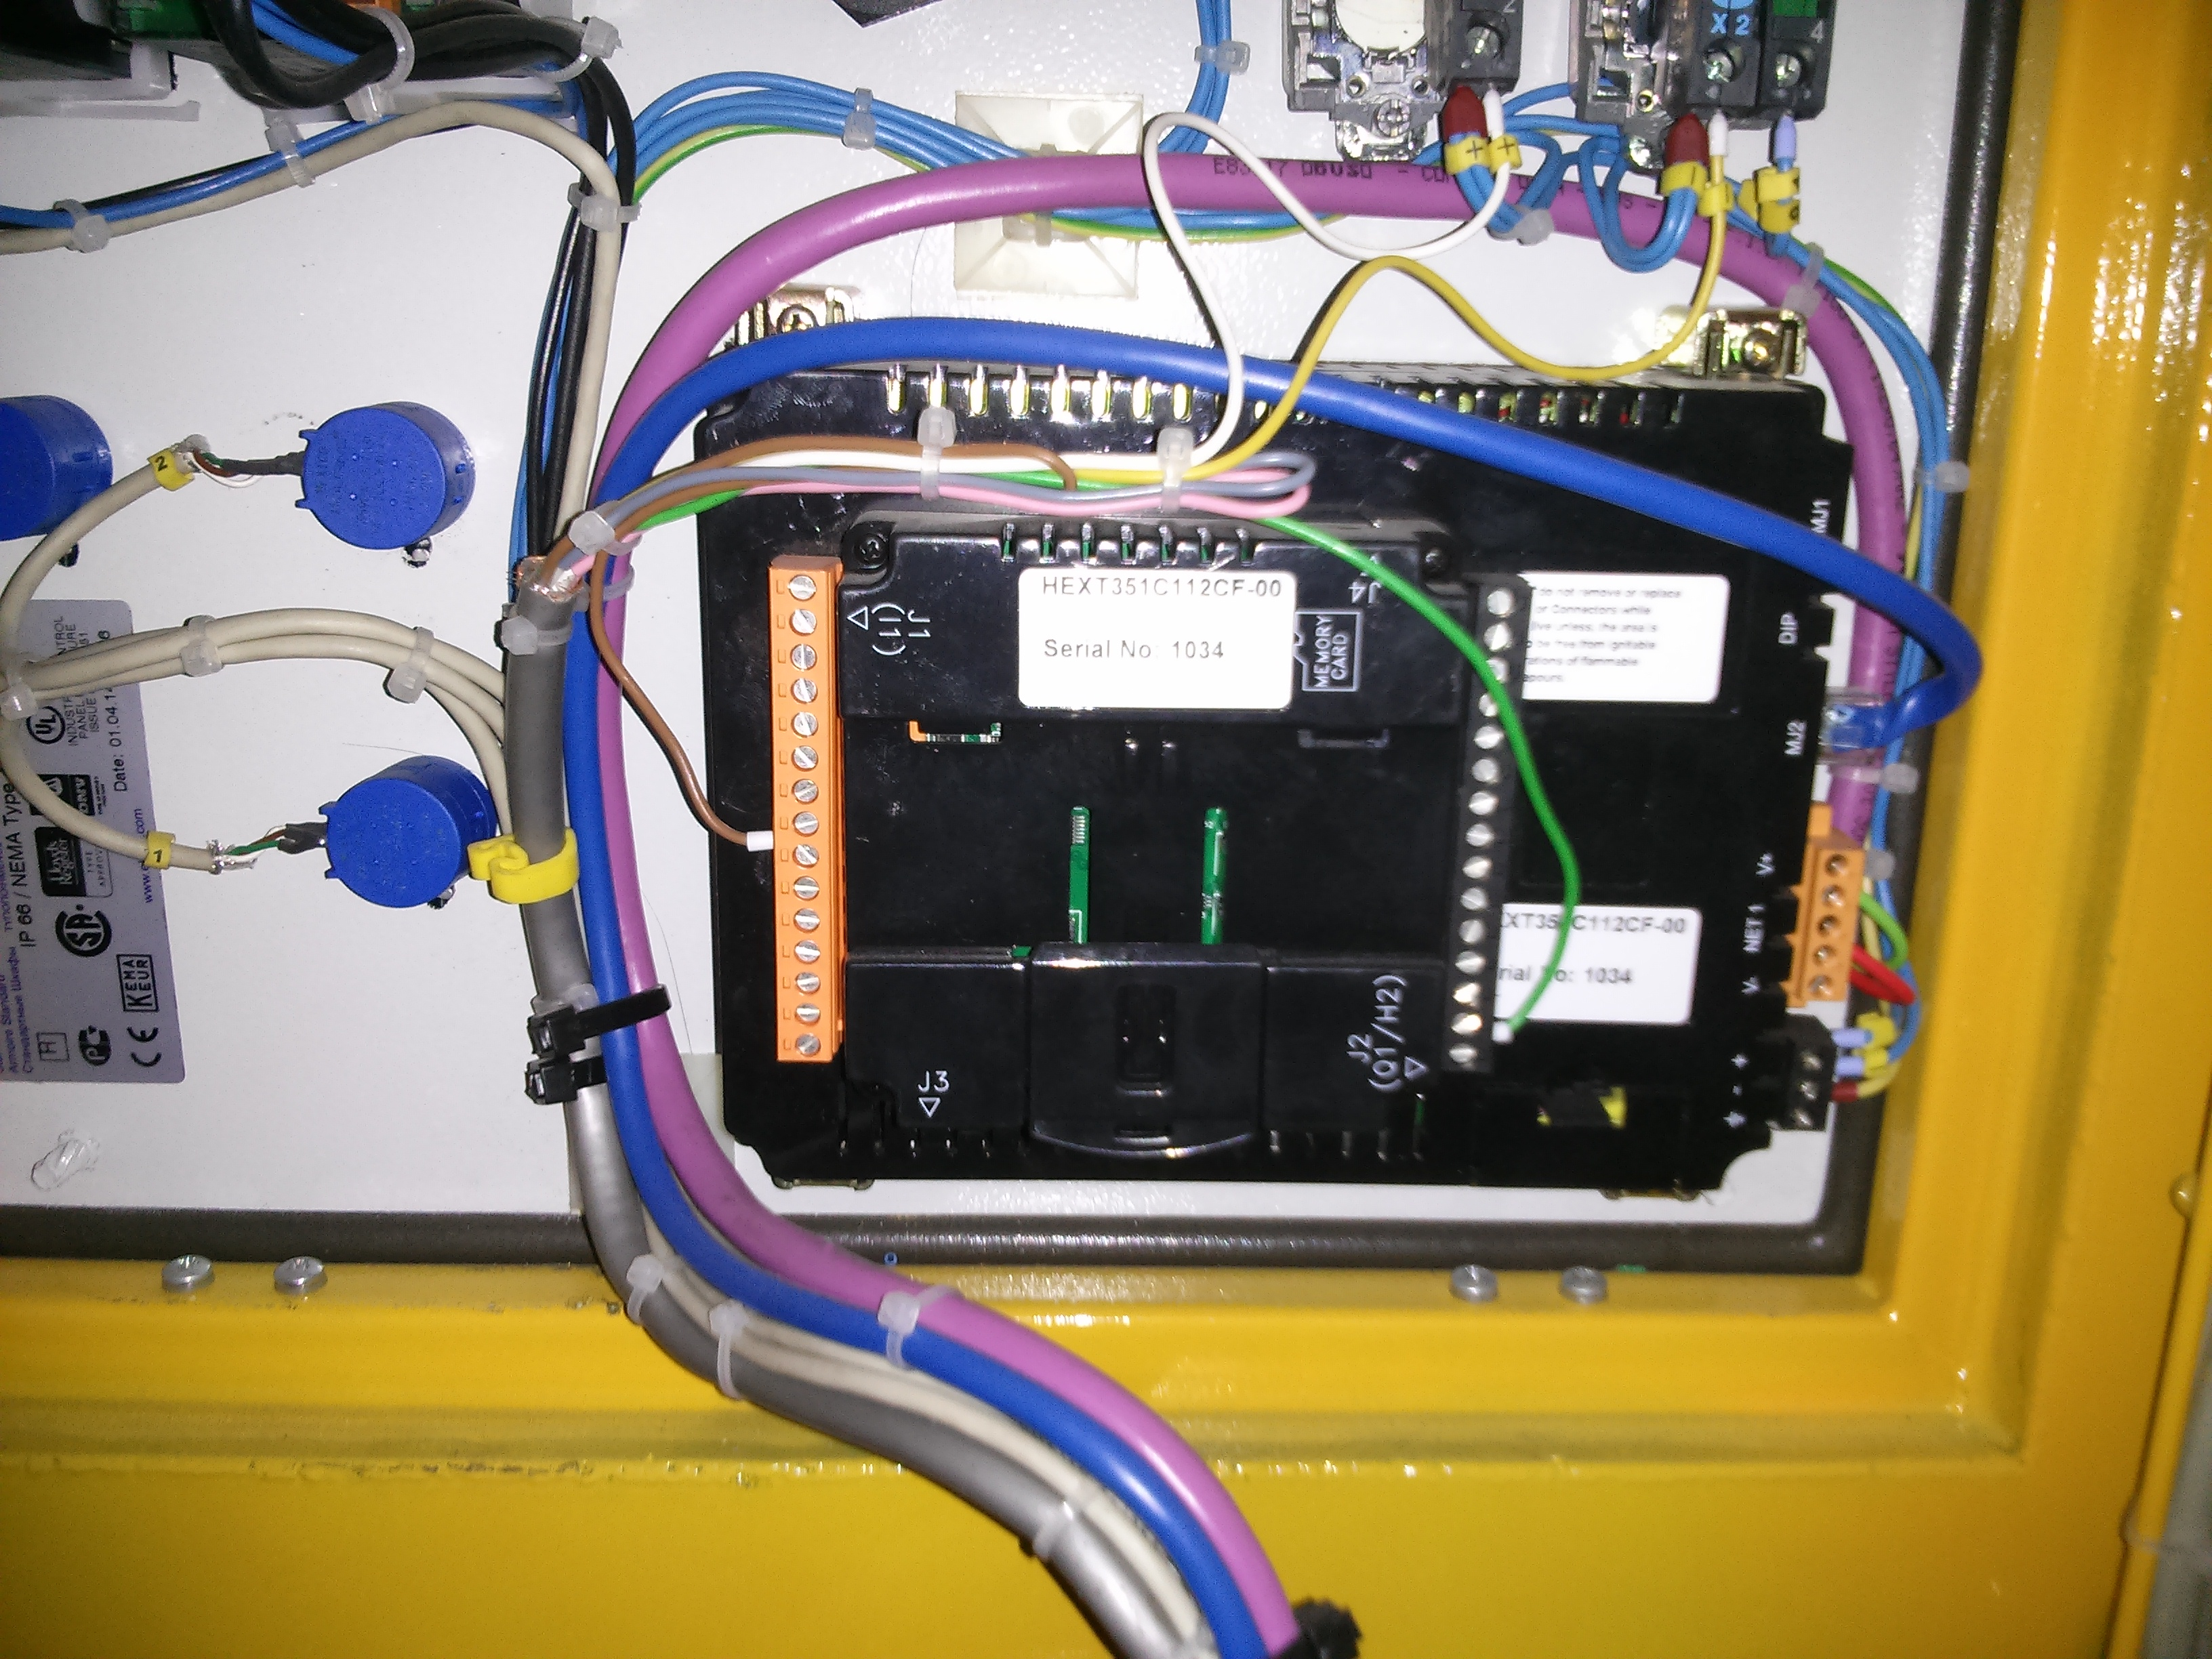
\includegraphics[width=0.4\textwidth]{images/huesca/IMG_20141216_175108.jpg}
            \caption{Pantalla HMI}
            \label{fig:hardware_HMI}
    \end{figure}

     \begin{figure}[H]
            \centering
            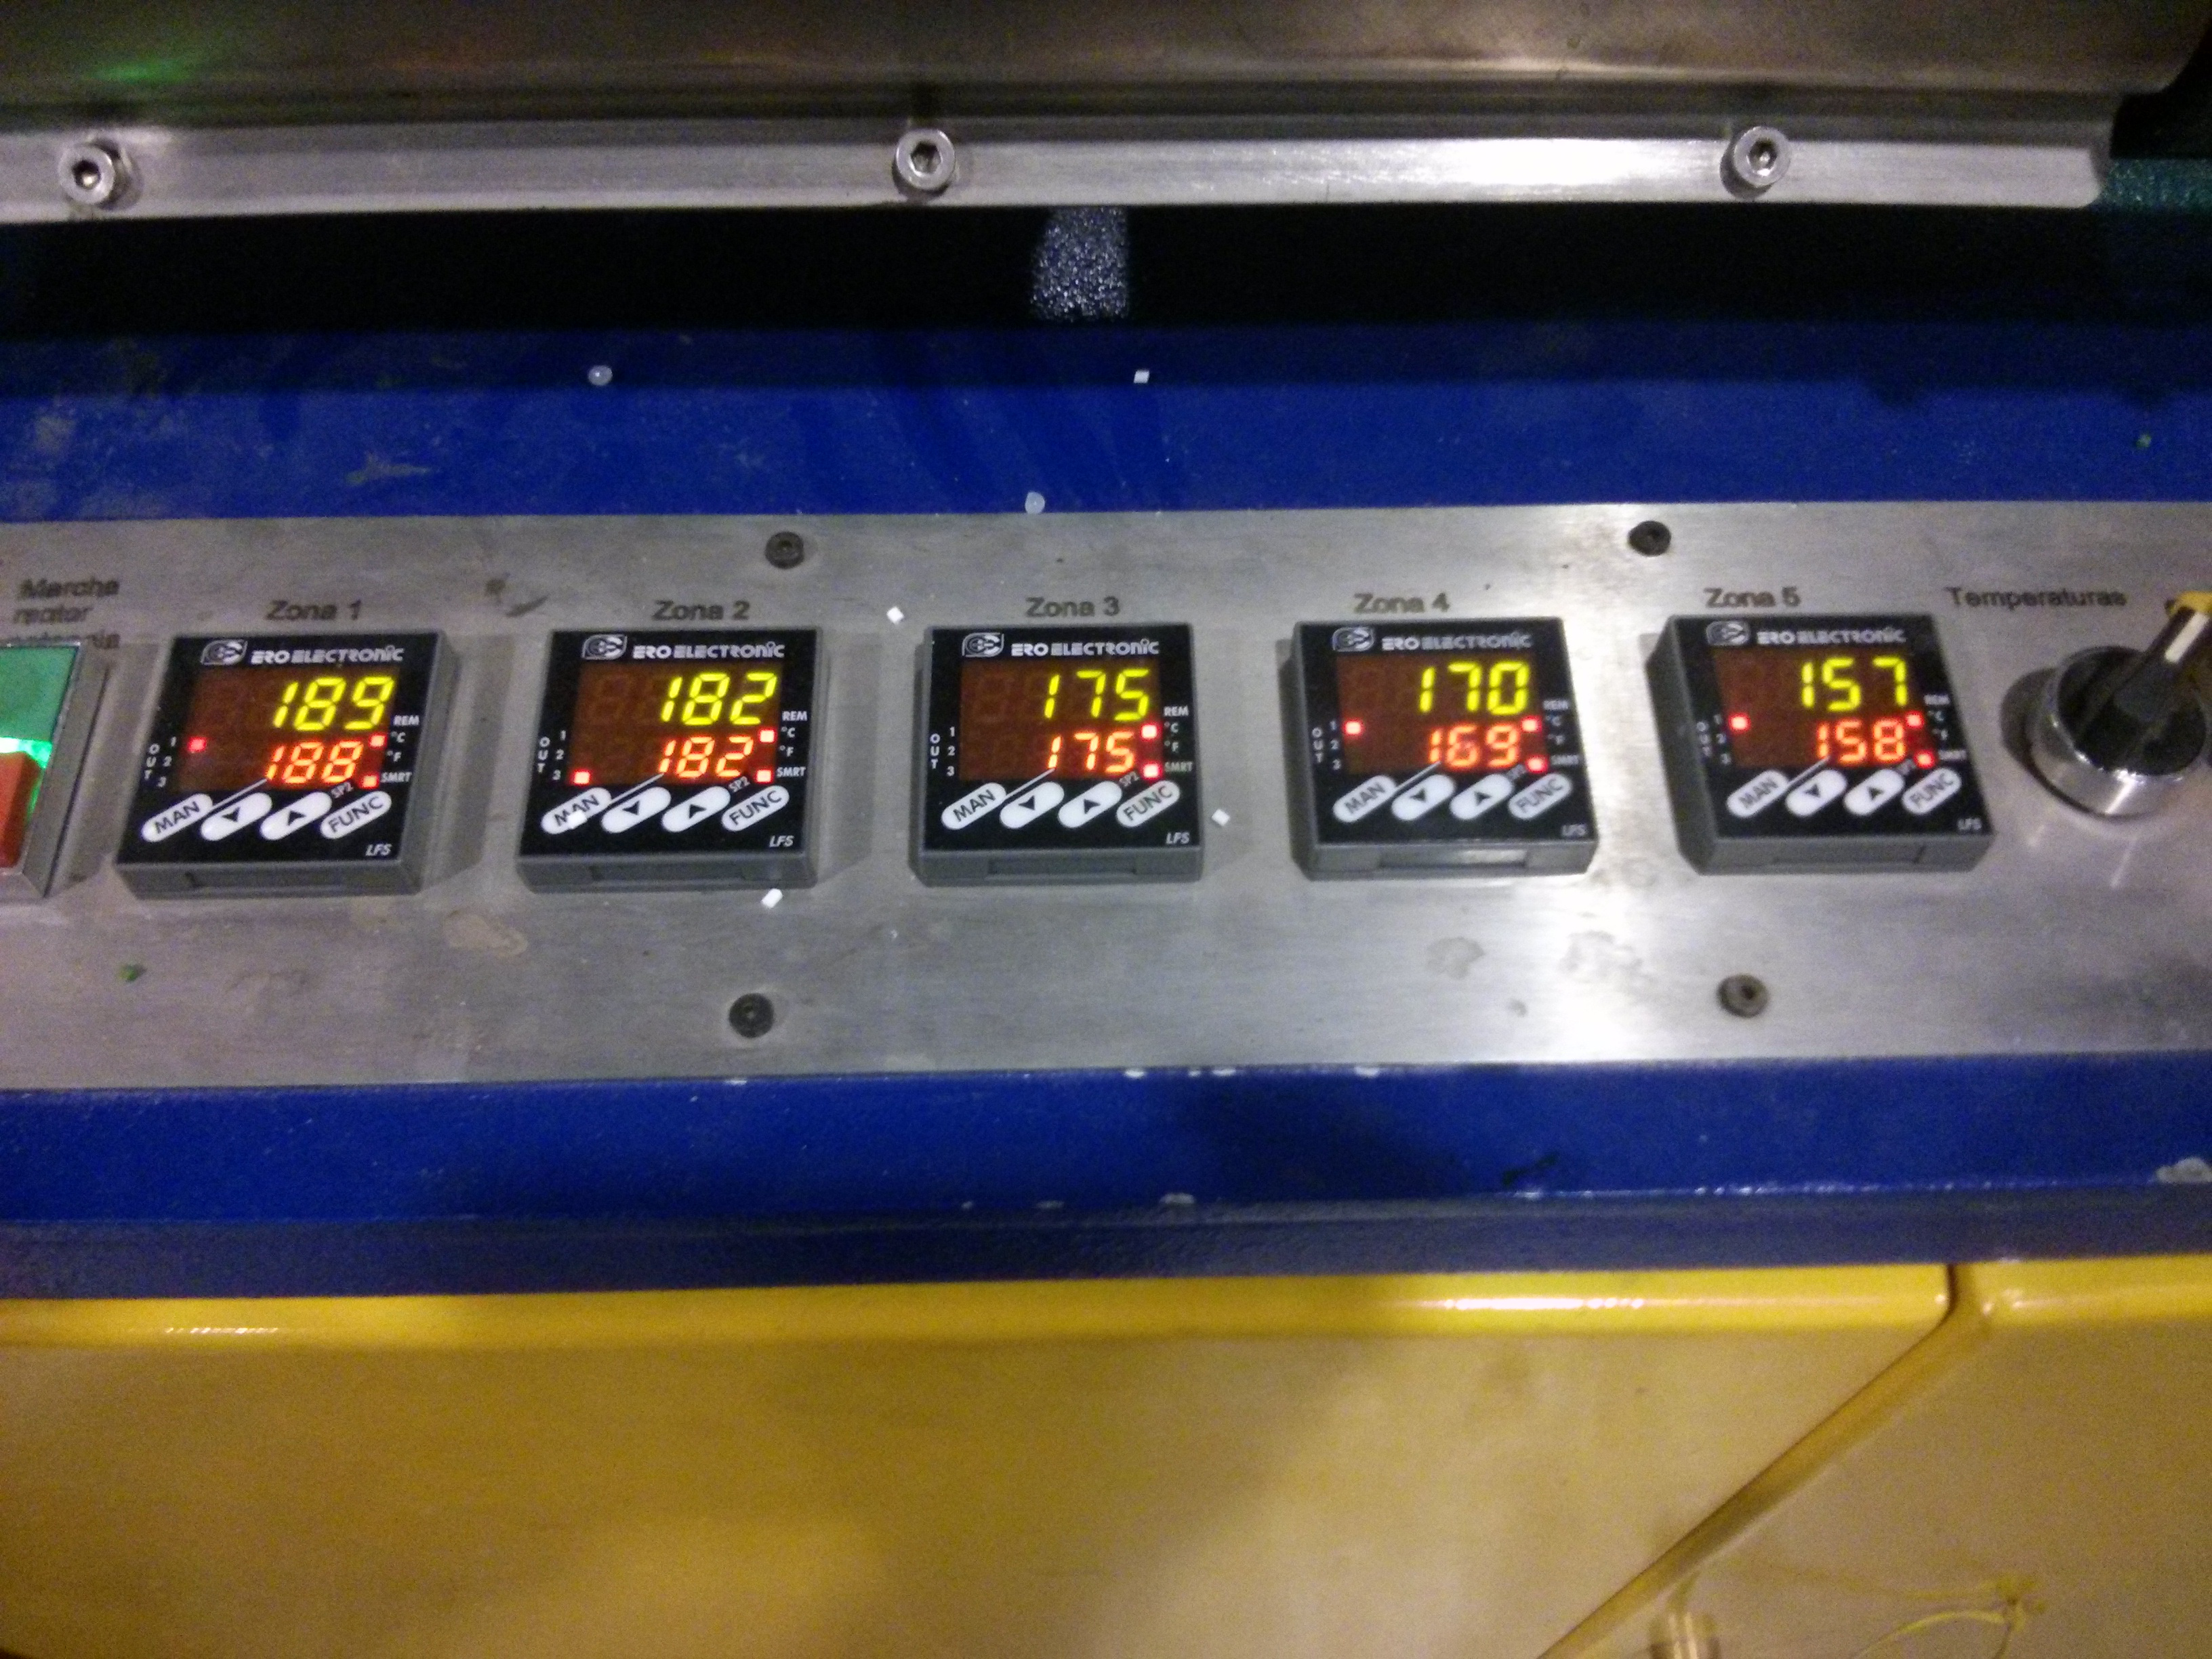
\includegraphics[width=0.4\textwidth]{images/huesca/IMG_20141216_175204.jpg}
            \caption{Sensores de temperatura}
            \label{fig:hardware_temperatura}
    \end{figure}

Buscando en internet referencias de los posibles componentes que disponemos, y con ayuda de los responsables de la fábrica, llegamos a la conclusión de que el hardware que disponemos es el siguiente:

\begin{itemize}
	\item \textbf{Reguladores temperatura Extrusora:} 5x Eroelectronic LFS
	\item \textbf{Regulador temperatura bañera:} 1x OMRON E5CC
	\item \textbf{Bobinadora: IO distribuidas: }
	\begin{itemize}

       \item {SmartStix I/O:} HE559DQM706B y HE559DI710B
       \item{HMI:} HE-XT351C112CF
        \item{Variador (control tractora):} Optidrive rrp2 ODP-24400-SP
        \item{Sensor diámetro:} conectado a módulo Adam 6066
        	\begin{itemize}
        				\item Omron ZX-GIF41 (RS232)
        				\item Omron ZX-GTC41 (Controlador)
                        \item Omron ZX-GT28S41 (sensor)
             \end{itemize}
        \item Relés: OMRON MY2IN
    \end{itemize}
\end{itemize}

Así mismo, disponemos de los datasheet y sabemos qué tipo de comunicación podemos disponer con cada uno, información necesaria para poder establecer la arquitectura del sistema.

\section{Arquitectura planteada}
\label{arquitectura}

Antes de plantear la arquitectura, deberemos establecer el protocolo de comunicaciones y el medio físico por el que irán conectados entre sí. El protocolo establece las reglas necesarias para que dos dispositivos se comuniquen correctamente, haciendo un simil con la realidad, sería el idioma que usan dos personas para hablar. Si dos personas mantienen una conversación en un distinto lenguaje, no se entenderán. Y el medio físico, es cómo se hará la comunicación. Mirando las especificaciones de los componentes llegamos a la siguiente conclusión

\begin{table}[H]

\begin{tabular}{ccc}
\hline
{\bf Dispositivo}     & {\bf Protocolo} & {\bf Medio} \\ \hline
Senores temperatura   & Modbus          & RS485       \\
Pantalla HMI          & Modbus          & RS485       \\
Adam                  & Modbus-TCP      & RS485       \\
Sensor diámetro       & -               & RS232       \\
Variador              & Modbus-TCP      & RS485       \\
Perifería distribuida & CsCAN           & Modbus      \\
Bobinadora            &                 & Cableado    \\ \hline
\end{tabular}
\centering
\caption{Dispositivos disponibles}
\label{tab:dispositivos}
\end{table}

Todos los dispositivos usan protocolos de comunicaciones industriales ampliamente conocidos, como son Modbus y CsCAN. El sensor de diámetro por ejemplo, está conectado a un PC mediante 
RS232, en el que almacena en una base de datos SQLITE (Ver imagen \ref{fig:hardware_sensor_diametro}) las medidas que se van tomando, por ello, será necesario acceder a esa base de datos.
 	\begin{figure}[H]
            \centering
            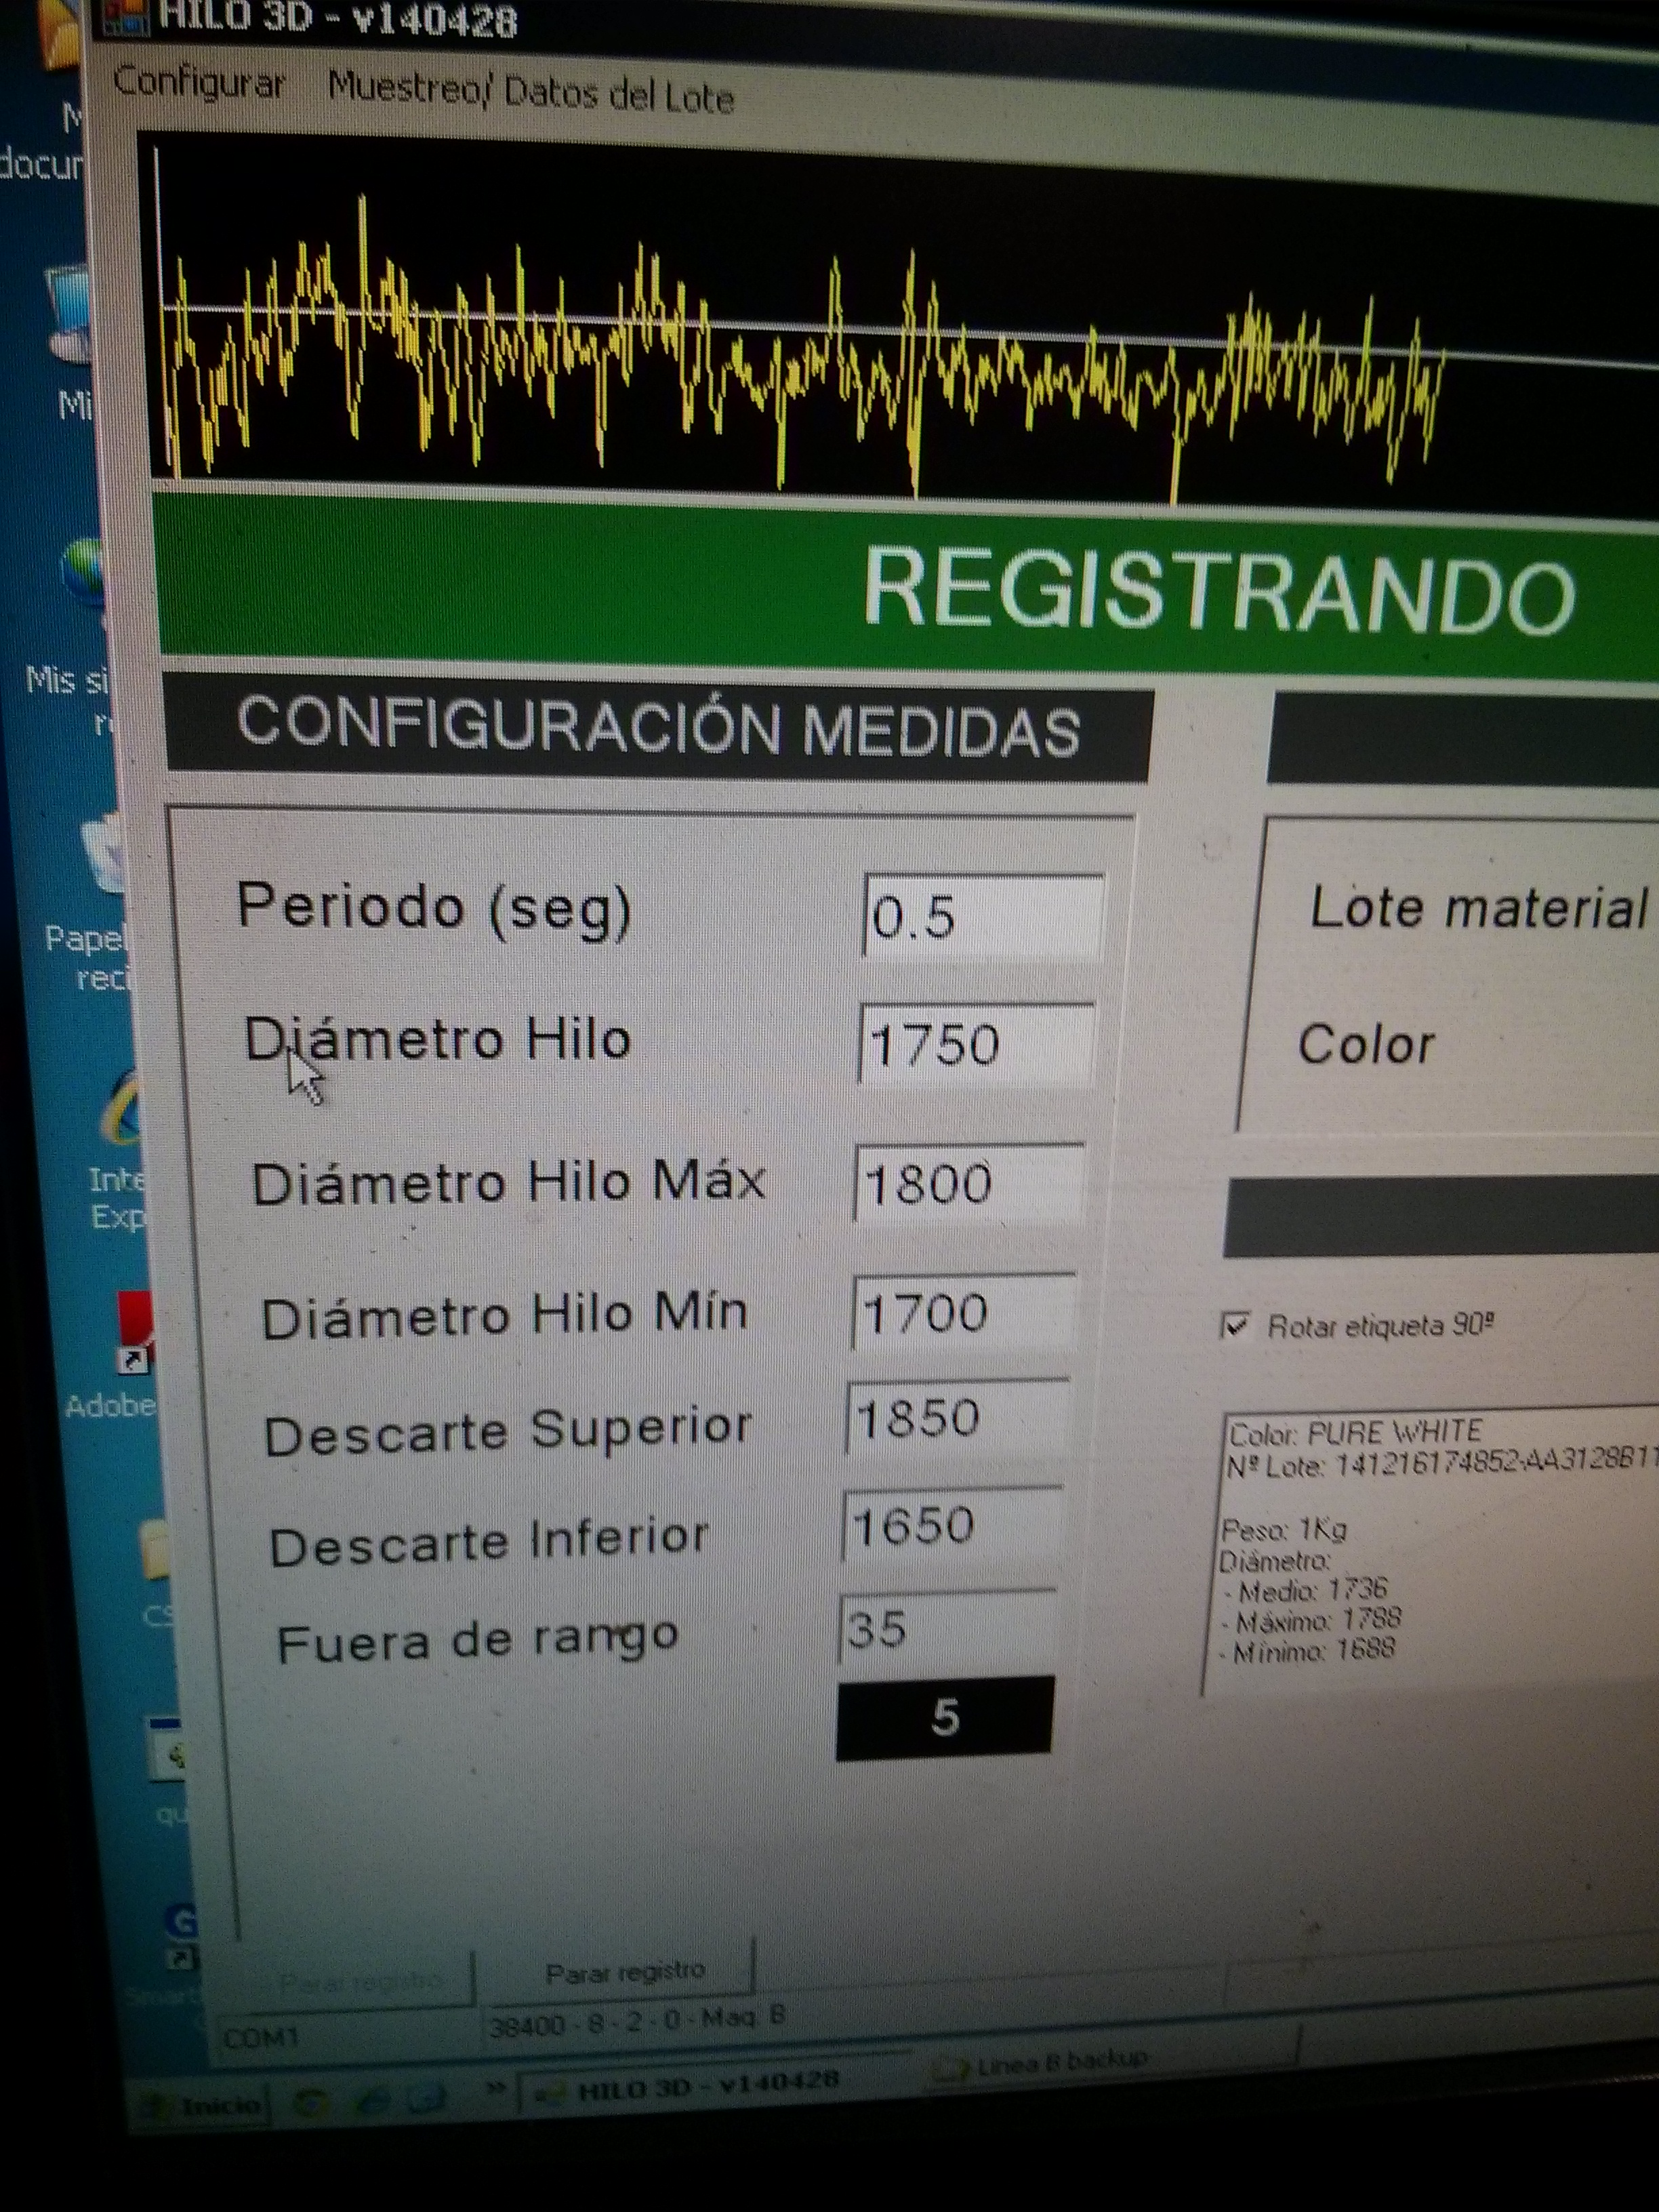
\includegraphics[width=0.5\textwidth]{images/Parametros_adquisicin.jpg}
            \caption{Programa que almacena las medidas tomadas en el sensor de diámetro}
            \label{fig:hardware_sensor_diametro}
    \end{figure}

La bobinadora, no usa ningún protocolo de comunicaciones, mediante señales de entrada salida, ese va realizando la comunicación.\\

Por tanto, con esta información, podemos establecer la arquitectura del sistema.\\

 	\begin{figure}[H]
            \centering
            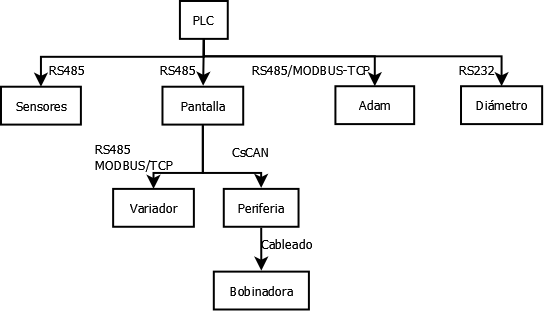
\includegraphics[width=0.6\textwidth]{images/20141229.png}
            \caption{Arquitectura propuesta}
            \label{fig:hardware_arquitectura}
    \end{figure}

Debemos buscar por tanto, un PLC que cumpla con las siguientes especificaciones:

% Please add the following required packages to your document preamble:
% \usepackage{multirow}
\begin{table}[H]
\centering
\begin{tabular}{|c|c|c|}
\hline
\textbf{Característica }                              & \textbf{Descripción}            & \textbf{Cantidad} \\ \hline
\multirow{3}{*}{Comunicaciones industriales} & Ethernet               & 1        \\ \cline{2-3} 
                                             & RS485                  & 1        \\ \cline{2-3} 
                                             & RS232                  & 1        \\ \hline
Software                                     & Acceso R/W a tabla SQL &          \\ \hline
Almacenamiento externo                       & USB o SD               & 1        \\ \hline
\multirow{2}{*}{Periferia digital}           & Entrada                & 8        \\ \cline{2-3} 
                                             & Salida                 & 0        \\ \hline
\multirow{2}{*}{Periferia analógica}         & Entrada                & 4        \\ \cline{2-3} 
                                             & Salida                 & 1        \\ \hline
\end{tabular}
\caption{Especificaciones PLC}
\label{tab:espc_plc}
\end{table}

\section{Elección del PLC}
\label{eleccion_PLC}

Se va a buscar un automáta programable (PLC) que cumpla las especificacione de la tabla \ref{tab:espc_plc}, también se intentará buscar una marca que nos ofrezca las siguientes ventajas, no siendo estas imprescindibles, pero si ayudarán a la hora de decantarnos por un modelo u otro:

\begin{itemize}
		\item{Licencia de desarrollo libre.}
		\item{Modelo básico con el mayor número de especificaciones necesarias.}
		\item{Capacidad de expansión de las características por medio de módulos.}
\end{itemize}

De este modo, conseguiremos reducir el coste total del proyecto. Partiendo de estos requisitos y buscando distintos proveedores por internet, las empresas que mejor se ajustan son:

\begin{itemize}
		\item{\textbf{UNITRONICS:} La compañía ofrece un PLC con pantalla HMI de bajo coste, que es idoneo para pequeños proyectos que no requieran demasiada capacidad. El principal problema es que no dispone de ningúna expansión para almacenar en tarjetas SD, ni se tiene conocimiendo de qu se pueda conectar a una bas de datos MYSQL de forma directa.}
		\item{\textbf{WAGO:} Cumple todos los requisitos que necesitamo, sin embargo, es necesario pagar una licencia para poder usar el software disponible}
		\item{\textbf{ABB:} El PLC de la gama eco trae de serie la mayoría de las cosas que necesitamos, además, si no se superan ciertas limitaciones, no es necesario pagar una licencia para poder usar el software de desarrollo.}
\end{itemize}

Se habla con cada uno de los distribuidores que ofrecen los productos en españa, pidiendo un presupuesto con el material necesario para suplir las necesidades del proyecto:

\begin{table}[H]
\centering
\begin{tabular}{cc}
{\bf Distribuidor} & {\bf Precio (\euro{})} \\ \hline
Unitronics         & 390              \\
Wago               & 1374             \\
Abb                & 506              \\ \hline
\end{tabular}
\caption{Presupuestos de los tres distribuidores}
\label{tab:presupuestos}
\end{table}


Debido al alto presupuesto que nos propuso Wago se descartó, ya que en una primera aproximación, se eligio ya que ofrecian alternativas baratas a grandes empresas como Siemens y ABB, sin embargo en el caso que nos ocupa y como se puede ver en la tabla \ref{tab:presupuestos} el precio de ABB es muy competitivo. De hecho es la marca que se elije, debido a que el coste con la marca Unitronics no supone un gasto excesivo y la fiabilidad de los automátas y el software que provee es mejor. Además trae de serie un servidor web con el que podremos hacer una interfaz WEB en la que veremos el estado de la fábrica de forma remota. Por ello, el hardware que se decide adquirir es el siguiente:

\begin{itemize}
	\item{PM564-RP-ETH CPU AC500-eCo,128kB,6DI/6DO-R/2AI/1AO, 24VDC. ETH y WEBSERVER. (Requiere: conectores 9+11 polos)}
\item{AI562 Módulo S500-eCo, 2AI PT100/1000, Ni100/1000, Resist. 150/300 ( Requiere conector 11 polos)}
\item{MC502 SD Memory Card 512 MB}
\item{MC503 Adaptador para tarjeta SD de memoria AC500-eCo.}

\end{itemize}

